\capitulo{4}{Técnicas y herramientas}
Para dar inicio a este capitulo, hay que entender la arquitecturadel proyecto. Para ello hay que pensar en como debe funcionar esta aplicación y como interactúa con el usuario.

eLearningQA interactúa con una API del servicio web de Moodle que le proporciona la mayoría de los datos de un curso de Moodle, esos datos se procesan para obtener resultados ilustrativos de la calidad de los cursos de Moodle, que se presentan en informes. 

\section{Modelo-Vista-Controlador}
La estructura de este proyecto sigue el patrón Modelo-Vista-Controlador\cite{mvc}. Este patrón arquitectónico divide el software en tres componentes:
\begin{itemize}
    \item \textbf{Modelo:} En este componentes se encuentran los datos y toda la lógica relativa a su obtención.
    \item \textbf{Vista:} En la vista se encuentra la interfaz gráfica y todos aquellos componentes que interactúen directamente con el usuario.
    \item \textbf{Controlador:} Este componente es el intermediario entre el modelo y la vista, este es el que gestiona las peticiones que se reciben de la vista y decide que datos mostrar y como, es decir, es el que contiene la lógica de negocio.
\end{itemize}

\begin{figure}[H]
    \centering
    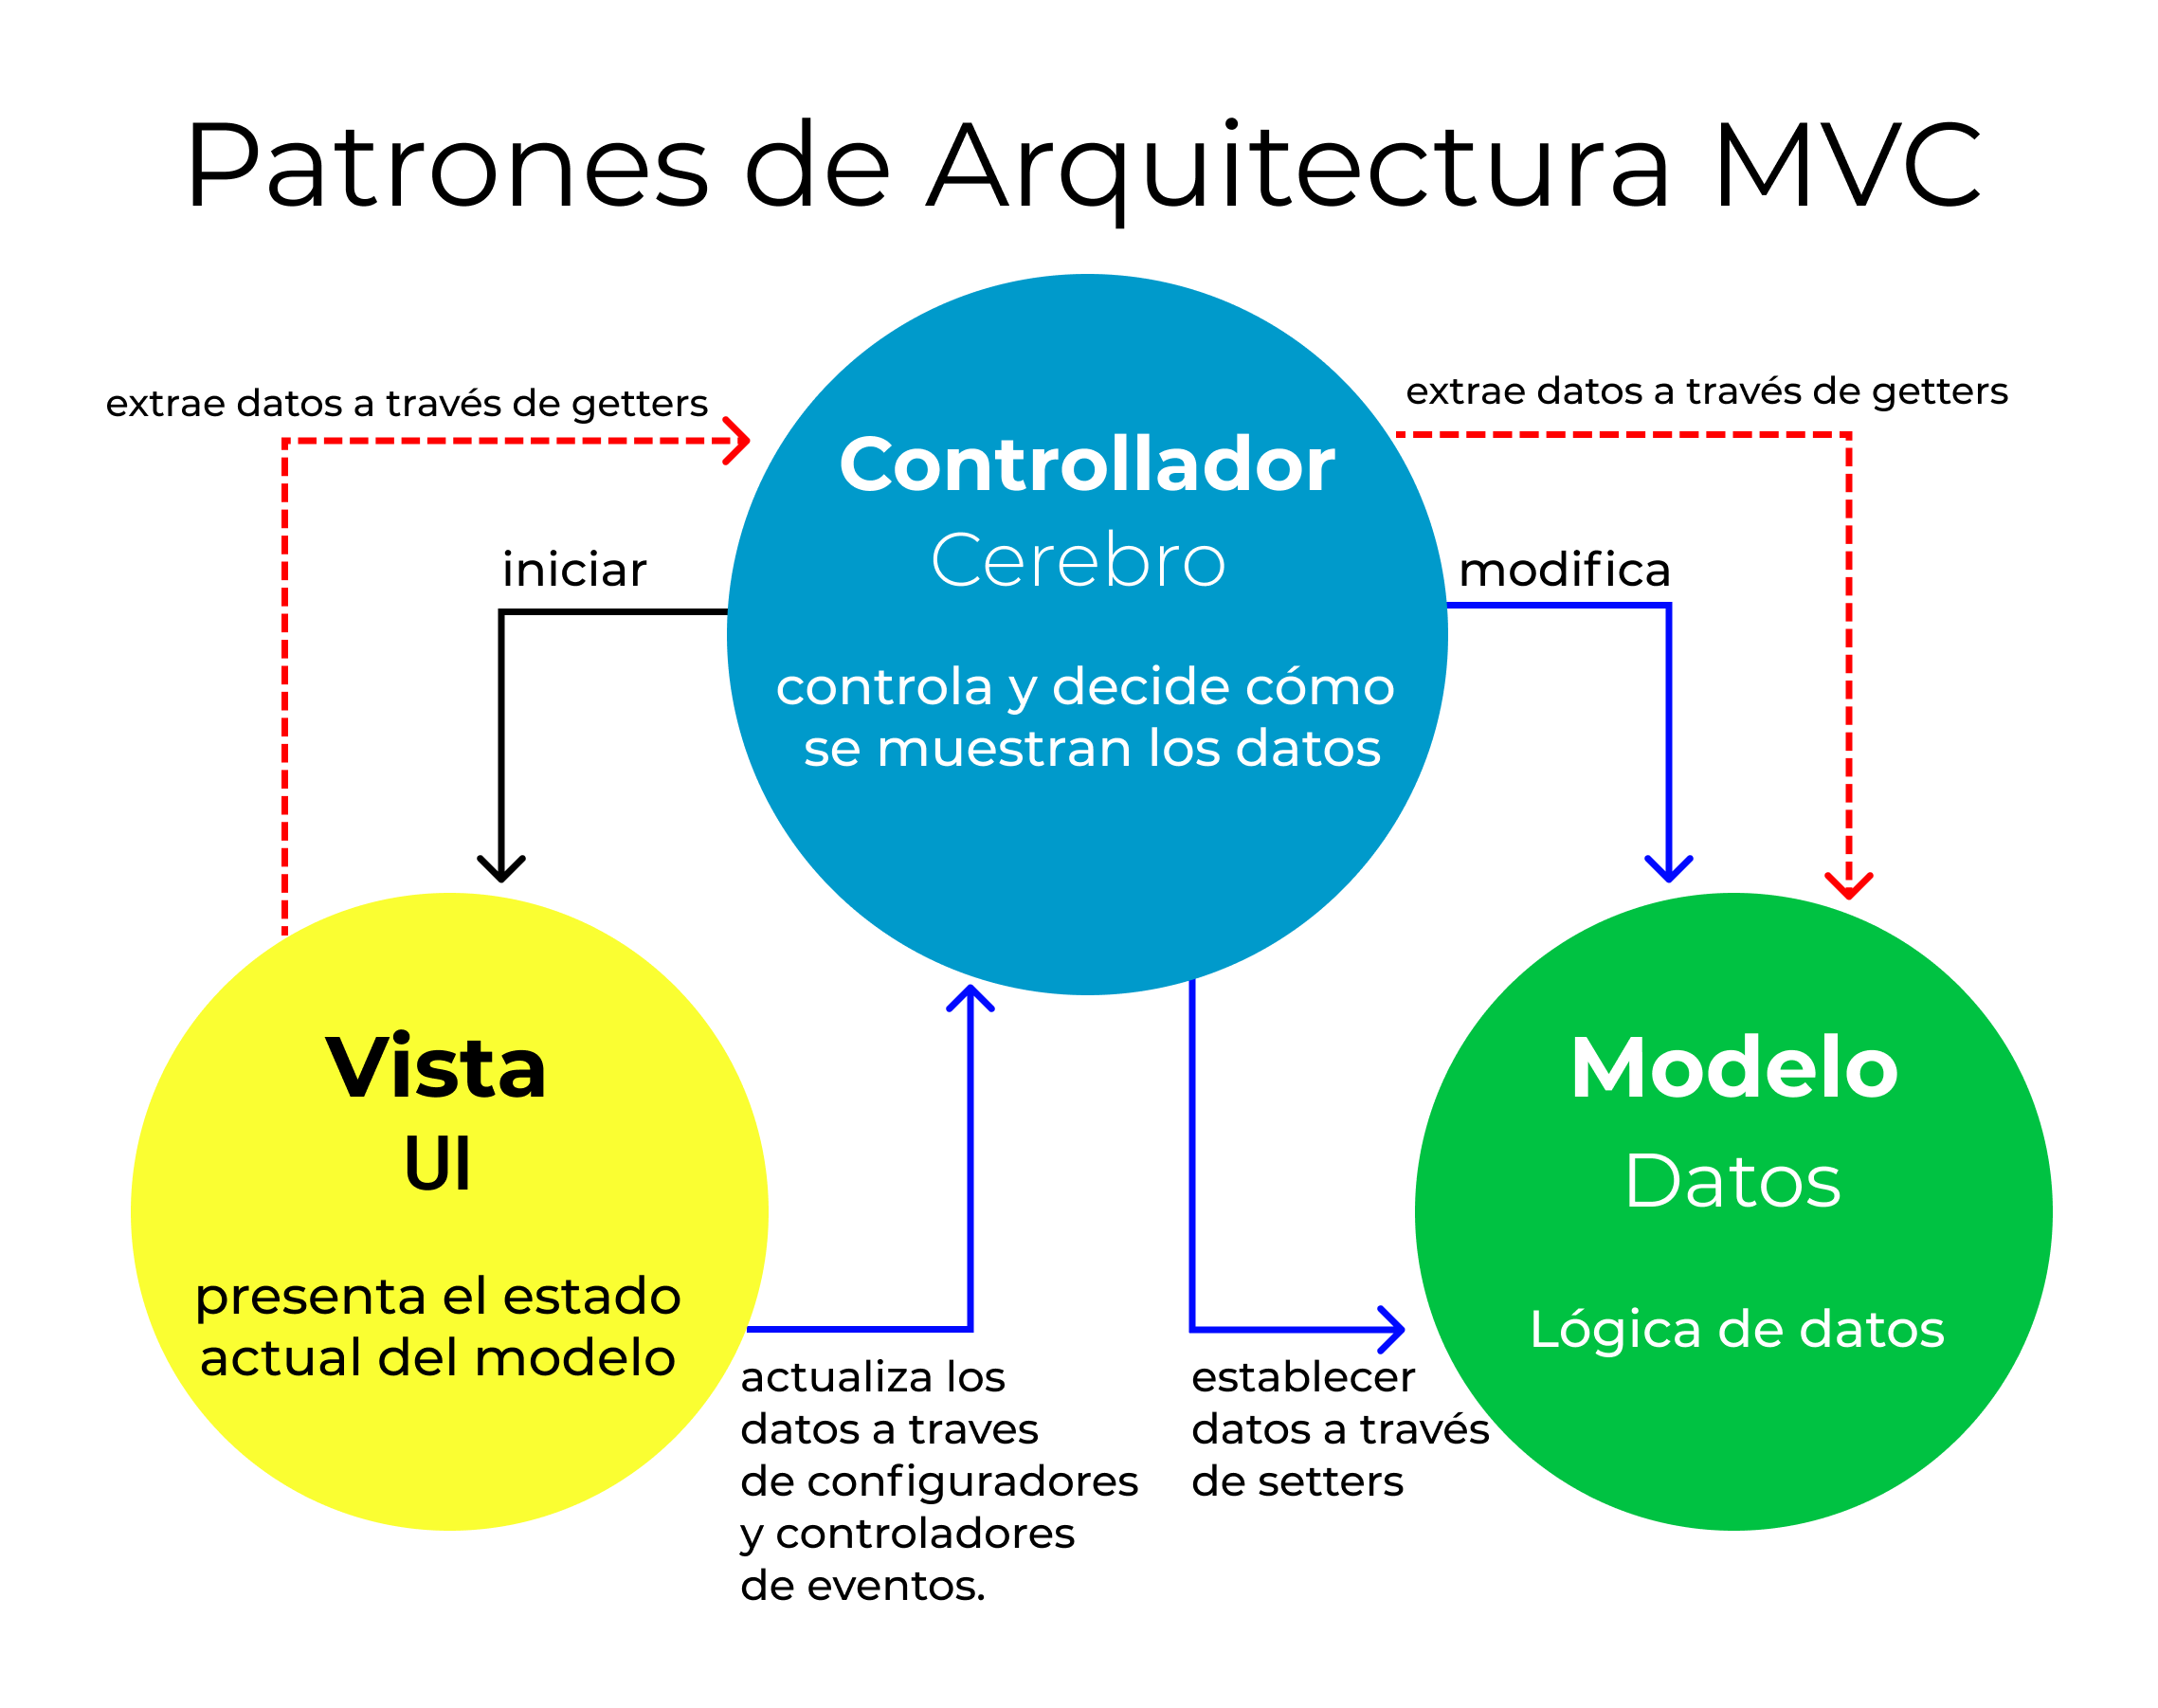
\includegraphics[width=0.80\linewidth]{img/MVC.png}
    \caption{Pátrón de arquitectura MVC}
    \label{fig:mvc-imagen}
\end{figure}

Con el patrón MVC \ref{fig:mvc-imagen} se pueden construir páginas web escalables mantenibles y fáciles de expandir. Además es una opción atractiva dado su facilidad de implementación y su clara divisón entre Frontend y Backend, lo que facilita la separación de preocupaciones.

\section{Técnicas utilizadas en el backend}
Una vez entendida la arquitectura del proyecto se puede profundizar a cada una de las partes que lo componen.

Empezando con el Backend, esta aplicación esta programada en Java utilizando Spring como framework y Maven para el control de dependencias. Además cuenta con contenerización con Docker.

\subsection{SpringBoot y Maven}
Spring Framework proporciona un modelo de configuración y programación intuitivo y fácil de usar. El objetivo de Spring Framework\cite{spring-framework} es realizar todas las configuraciones internas necesarias para que los equipos de desarrollo solo tengan que encargarse de desarrollar la lógica de negocio y no dediquen excesivo tiempo a la configuración del proyecto.

Uno de los proyectos que ofrece Spring es SpringBoot\cite{spring-boot} que permite crear stand-alone y ejecutarlas rápidamente. Además, cuenta con servidores web embebidos lo que facilita enormemente el desarrollo de una aplicación web.

Para proveer de SpringBoot y de todas las dependencias que necesita esta aplicación se utiliza Maven que proporciona un fichero xml llamado POM que permite añadir todas las dependencias necesarias al proyecto fácilmente.

\subsection{Docker}
Docker \cite{docker} es una plataforma de desarrollo que permite desacoplar las aplicaciones de la infraestructura de forma que se puede enviar y desplegar aplicaciones rápidamente. Docker se basa en la contenerización \cite{contenerización}. 

La contenerización consiste en que las aplicaciones son empaquetadas con aquellas bibliotecas del sistema operativo necesarias para que se ejecute, de esta forma se pueden desplegar aplicaciones en cualquier sitio de forma rápida y ligera.

\begin{figure}[H]
    \centering
    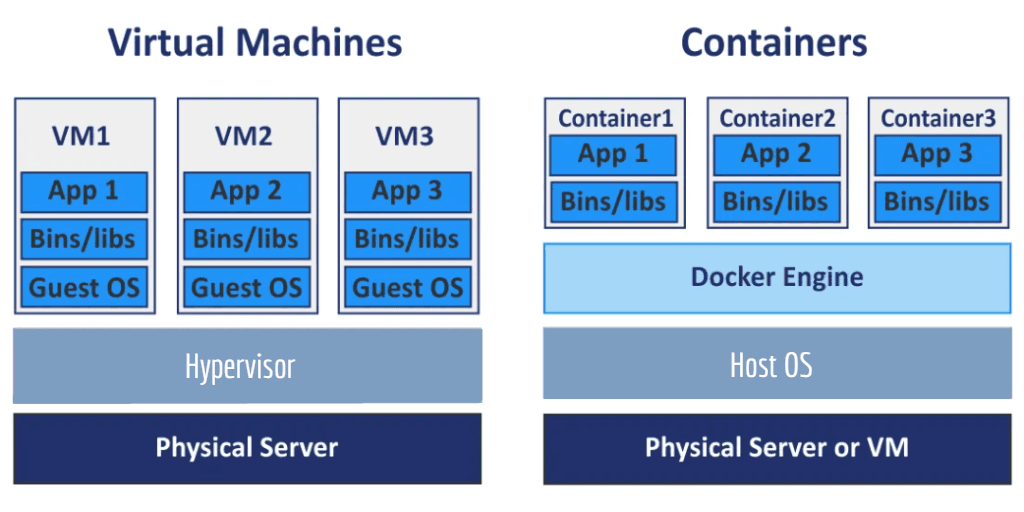
\includegraphics[width=0.80\linewidth]{img/docker-vs-vm.png}
    \caption{Contenerización con Docker vs virtualización}
    \label{fig:docker-imagen}
\end{figure}

En la imagen anterior \ref{fig:docker-imagen}, se puede ver claramente la diferencia de los contenedores con las máquinas virtuales. Se puede ver que con los contenedores se ejecutan sobre la misma ``maquina'' compartiendo sistema operativo, mientras que con las máquinas virtuales cada aplicación se ejecuta en un sistema operativo.

Docker se ha implementado al proyecto \cite{dockerizar-entorno} utilizando principalmente el .war que se genera al compilar la aplicación. Con este .war, que lleva embebido un servidor Tomcat, se puede crear una Dockerfile que ejecute el .war compilado con el siguiente comando:
    \begin{verbatim}
        java -jar prototipo-0.4-SNAPSHOT.war
    \end{verbatim}
Con esto, se obtiene una imagen que debe ser ejecutada en un contenedor. 
\section{Técnicas utilizadas en el frontend}
El frontend se entiende como todos los componentes que interactúan directamente con el usuario y la lógica en ellos. Actualmente, existe una gran variedad de opciónes para implementar el frontend de una aplicación, tales como, Angular \cite{angular}, React \cite{react} o Vue.js \cite{vue}.

En el caso de eLearningQA, se utiliza JSP (Java Server Pages) \cite{jsp}. Las páginas JSP \ref{fig:diagrama-jsp}  son una mezcla de código HTML, XML y Java que son convertidas a un servlet el cual genera la vista. Existen opciones más sencillas de implementar y con más capacidades como las nombradas anteriormente. Sin embargo, para hacer interfaces básicas y rápidamente es una buena opción.

\begin{figure}[H]
    \centering
    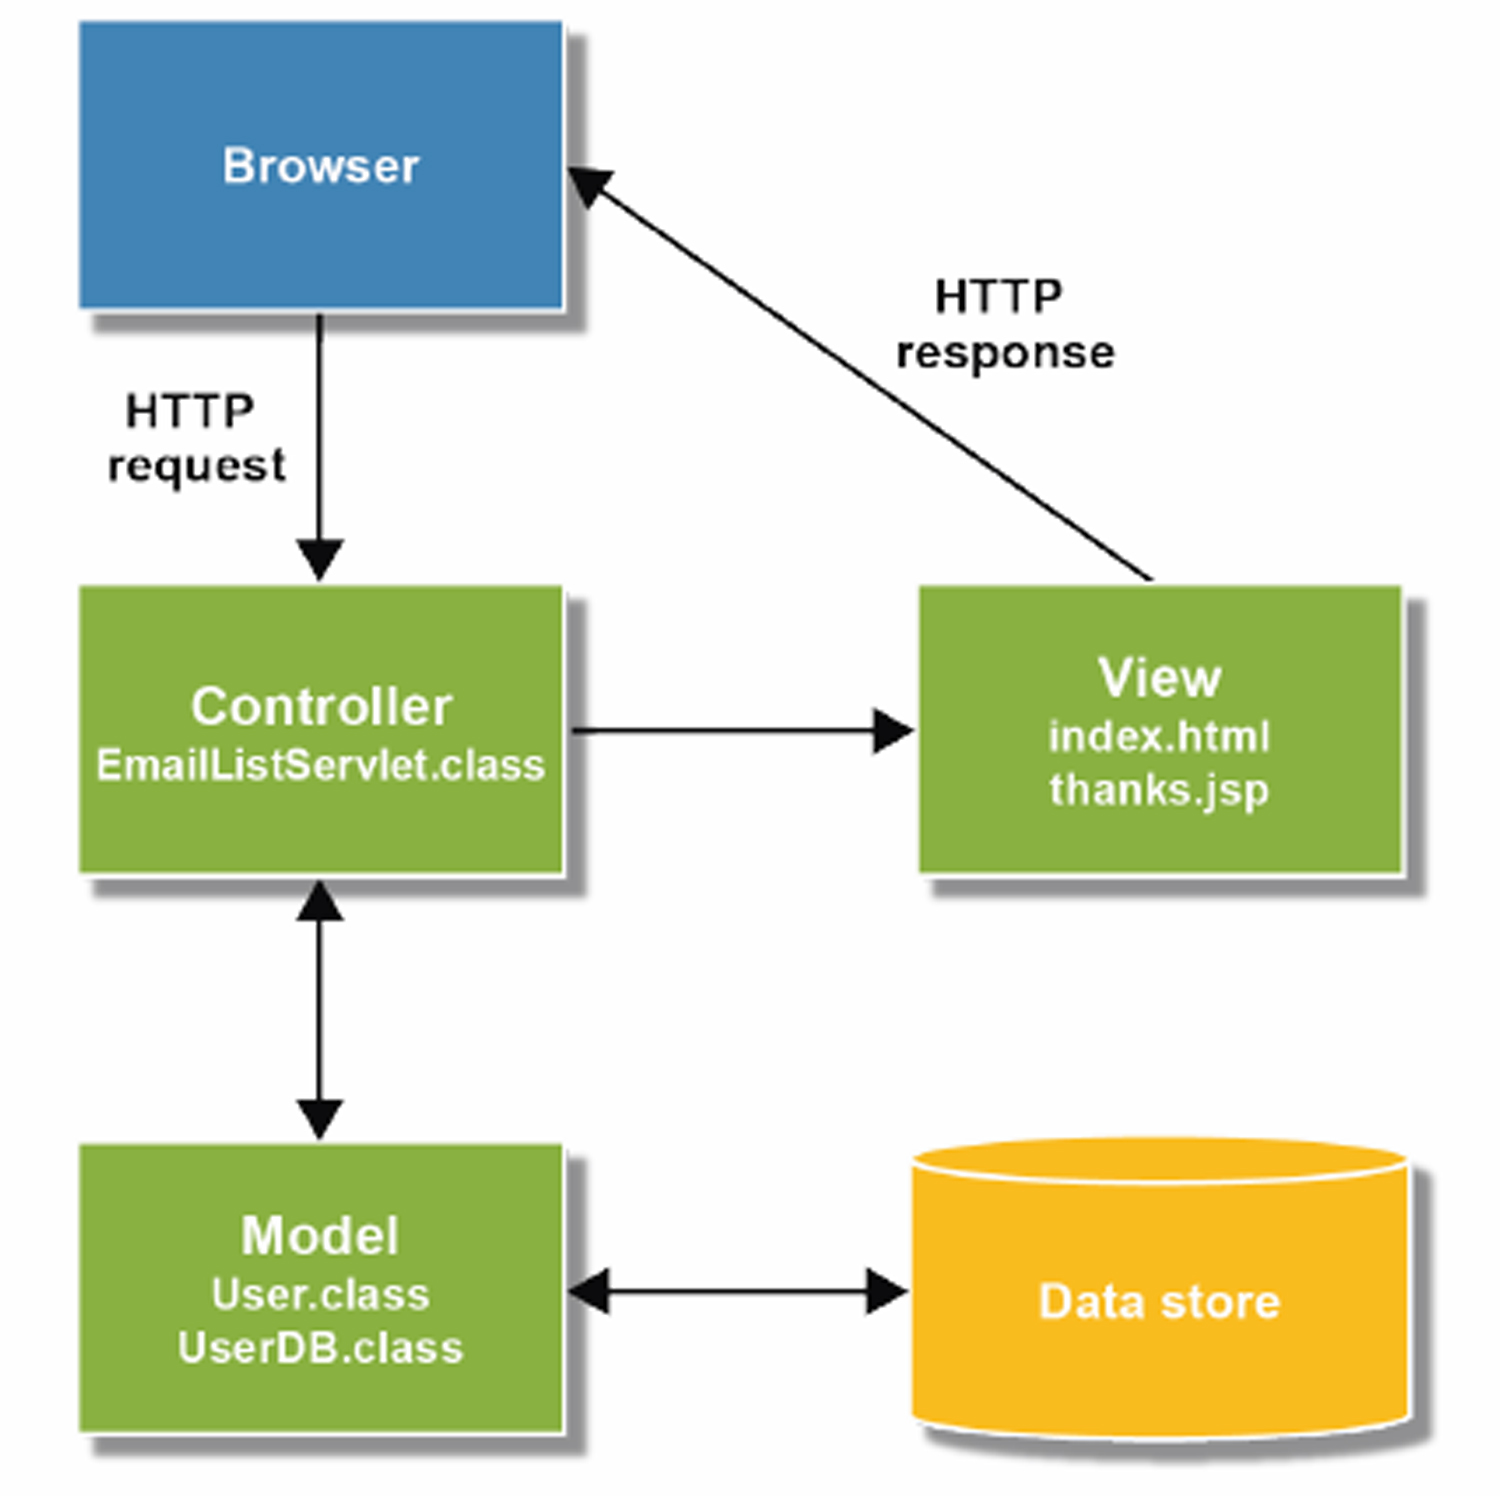
\includegraphics[width=0.65\linewidth]{img/servlet.jpg}
    \caption{Funcionamiento del Servlet y JSP}
    \label{fig:diagrama-jsp}
\end{figure}
    
\section{Modelo de desarrollo software}
El modelo de desarrollo software es un enfoque sistemático que describe todas las actividades del ciclo de vida del desarrollo software. Existen varios enfoques \cite{modelo-desarrollo} pero el que se ha aplicado en el desarrollo de este proyecto ha sido el modelo ágil.

\subsection{Modelo ágil}
Este modelo se basa en la adaptabilidad, la colaboración y el desarrollo incremental. Además con este modelo fomenta la entrega rápida del software cosa muy valorada en este proyecto.

El modelo ágil consiste en la división del trabajo en iteraciones cortas llamadas sprint. Antes de cada sprint se asigna una cantidad de trabajo a cada participante en orden de prioridad. Cuando comienza el sprint se realiza el trabajo y se realizan reuniones diarias con el equipo para hacer un seguimiento de los avances. A medida que se terminan funcionalidades se integran y se realizan pruebas. Cuando termina el sprint se realiza una revisión de todas las tareas completadas y todos los miembros del equipo hacen sus comentarios sobre el sprint. 

Para aplicar esta metodología existen herramientas como Jira o Zube, que facilitan el trabajo del project manger, que sería el encargado de la gestión del equipo. En el caso de este proyecto, se ha utilizado Zube.io para aplicar la metodología ágil, de forma que los miembros del equipo podían subir sus avances y cuestiones, además de monitorizar sus avances con herramientas analíticas que ofrece Zube.io.

\begin{figure}[H]
    \centering
    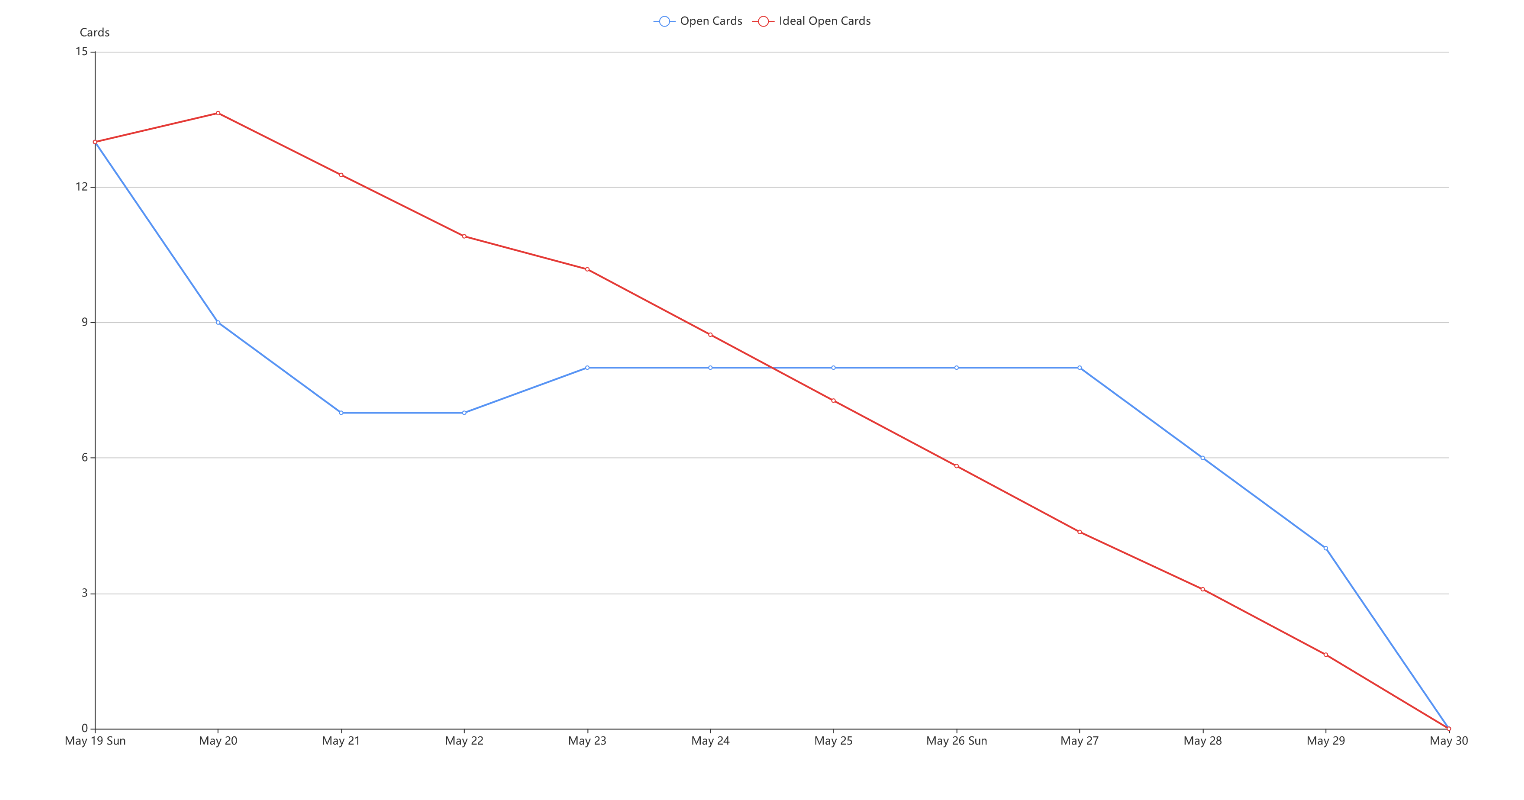
\includegraphics[width=1\linewidth]{sprint-burndown.png}
    \caption{Analítica de burndown de un sprint del proyecto}
    \label{fig:enter-label}
\end{figure}

\subsection{Repositorio de proyecto y sistemas de control de versiones}
Para hacer un desarrollo sostenible y seguro es conveniente contar con un controlador de versiones, que no solo asegura que exista una copia de un proyecto en algún lugar, si no que permite a los miembros de un equipo trabajar en paralelo de forma rápida y cómoda. Además permite implementar CI/CD, que hace que el desarrollo y la integración sea rápida y segura.

La elección para el controlador de versiones de este proyecto es GitHub, que gracias a su facilidad de uso y a las posibilidades que ofrece facilita y mejora el desarrollo de aplicaciones.

Además, Github ofrece la posibilidad de llevar a cabo CI/CD \cite{ci-cd} con las GitHub Actions. La integración continua y la entrega continua son fases por las que pasan los productos software para hacer una entrega de producto continuo y sin errores. En este proyecto se utiliza el Java CI con Maven, esto se utiliza para hacer una complicación con Maven en cada commit, si la compilación ha ido correctamente el desarrollador podrá seguir con sus tareas, sin embargo, si ha habido errores en esa compilación sera necesario tomar medidas correctivas para que el proyecto no tenga errores en remoto.

\begin{figure}[H]
    \centering
    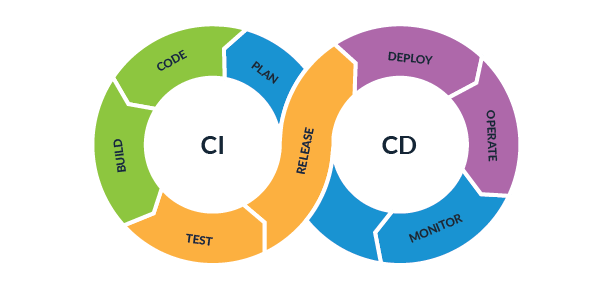
\includegraphics[width=1\linewidth]{img/ci-cd.png}
    \caption{Esquema ilustrativo de CI/CD}
    \label{fig:enter-label}
\end{figure}

Como conclusión, también es interesante añadir que con GitHub es posible conectar proyectos a herramientas de calidad como SonarCloud que pueden ayudar al mantenimiento de calidad del proyecto.

\subsection{SonarCloud}
SonarCloud \cite{sonar-cloud} es una herramienta que proporciona un amplio análisis de código y que permite a los desarrolladores conocer datos importantes sobre el código que están desarrollando como cobertura de test, brechas de seguridad, complejidad visual, duplicación de código, etc.

En este proyecto se utiliza SonarCloud para hacer un desarrollo sostenible, seguro y consistente. De forma que todas las personas que aporten en el desarrollo del código de la aplicación hagan un trabajo pulcro y consistente con el trabajo de los demás. SonarCloud, además, ayuda a evitar posibles brechas en la seguridad que pondrían en una mala posición tanto a desarrolladores como a clientes. El sonarQube de este proyecto se encuentra en


